\section{Top-bottom approach} % (fold)
\label{sec:top_bottom_approach}
	This chapter will cover the last step in our methodology: going back from the modified model to the physical system, while applying the introduced modifications.

	This is a Top-bottom approach, which is of growing interests nowadays. This method becomes interesting when the behavior of the low-level parts is hard to create, when the global behavior does not simply follow from the behavior of the low-level parts or when we want to low-level parts to follow directives given at a higher level.

	In our case, our problem is that we do not know how to modify the behavior of the low-level parts (i.e. the robots and pieces and their interactions) so as to create a high-level goal. When working on the mathematical model level, we can define our high-level goals more easily.

	The main difficulty of this approach is to create a mapping from the high-level to the low-level.
% section top_bottom_approach (end)

\section{Rates mapping} % (fold)
\label{sec:rates_mapping}
	In our case, this problem is actually simpler, because we have a direct dependance between rates in the mathematical model and behavior of the robots.
	
	Especially, we created a bidirectional relation between the stochastic constant rates of our mathematical model and physical capacities or behavior of our robots and pieces. The mapping from the model to the physical system is thus straightforward:
	\begin{description}
		\item[Backward probability $p_i^-$:] A robot carrying an assembly draws a random number at each timestep and compare it to the $p_i^-$ corresponding to its carried assembly $i$. Precisely:
		
		\textit{if} $U(0,1) < p_i^-\cdot T \rightarrow $ \textit{disasssemble assembly} $i$.
		
		where $T$ is the timestep of the physical simulation. This is needed because $p_i^-$ is a backward rate per second.
		\item[Forward probability $p_i^+$:] As shown in Equation~\eqref{eq:forward_rate_opt}, this probability is used when an assembly is starting. Before actually doing the assembly, a random number is drawn and compared to it:
		
		\textit{if} $U(0,1) < p_i^+\cdot T \rightarrow $ \textit{perform assembly step} $i$.
	\end{description}
	
	When a disassembly is triggered, the carrying robot drops one of the assemblies on the ground and resume searching with the remaining carried assembly. This dropped assembly should then be grabbed by another robot in order to be attached again.
	
	These behavior should directly create the change of rates needed for the modified mathematical model.
	
	When such a bidirectional mapping is not that easily available, we have to discover that mapping. A possibility would be to create an iterative process between a modification of low-level parameters and a measure of the resulting rate modification in the model.
% section rates_mapping (end)

\section{Augmentation results and implications} % (fold)
\label{sec:augmentation_results_and_implications}

	We choose to implement the set of optimized probabilities shown in Table~\ref{tab:optimized_probabilities_augmented}. It has been found by solving problem P1 in Section~\ref{sec:results_and_limitations}.
	
	\begin{table}
		\begin{center}
		\begin{tabular}{|c|c|c|c|c|c|c|c|}
			\hline
			\multicolumn{2}{|c|}{\textbf{Reaction} $\mathbf{j}$} & \textbf{1} & \textbf{2} & \textbf{3} & \textbf{4} & \textbf{5} & \textbf{6} \\
			\hline
			 	& $\alpha = 0.01$ & \multicolumn{6}{c|}{} \\
			$\mathbf{p^+_j}$ & $\alpha = 0.5$ & \multicolumn{6}{c|}{1.0} \\
				& $\alpha = 0.99$ & \multicolumn{6}{c|}{} \\
			\hline
			& $\alpha = 0.01$ &  &  &  & 0.033074 &  & 0.000134 \\
			$\mathbf{p^-_j}$ & $\alpha = 0.5$ & 0.018852 & 0.007541 & 0.003770 & 0.000661 & 0.009426 & 0.000265 \\
			& $\alpha = 0.99$ &  &  &  &  0.000334 &  & 0.013229 \\
			\hline
		\end{tabular}
		\end{center}
		\caption{Set of optimized probabilities used for the Top-down mapping. Reactions from system \eqref{eq:modified_system:reactions}.}
		\label{tab:optimized_probabilities_augmented}
	\end{table}
	
	\subsection{Stochastic model} % (fold)
	\label{sub:stochastic_model}
		We start by verifying the behavior with the stochastic simulation of our model with backward rates. We modify Equation~\eqref{eq:ode_transportersimple} to add the backward reactions while still modeling the robots and free pieces. Our model takes into account the dropped pieces when a disassembly occurs. The results for 1 puzzle are shown in Figure~\ref{fig:stoch_augm_1puzzle}. The results are similar for 3 puzzles, so we do not show them here.
		
			\begin{figure}[h!]
				%\centering
				\subfigure[$\alpha = 0.01$] 
				{
					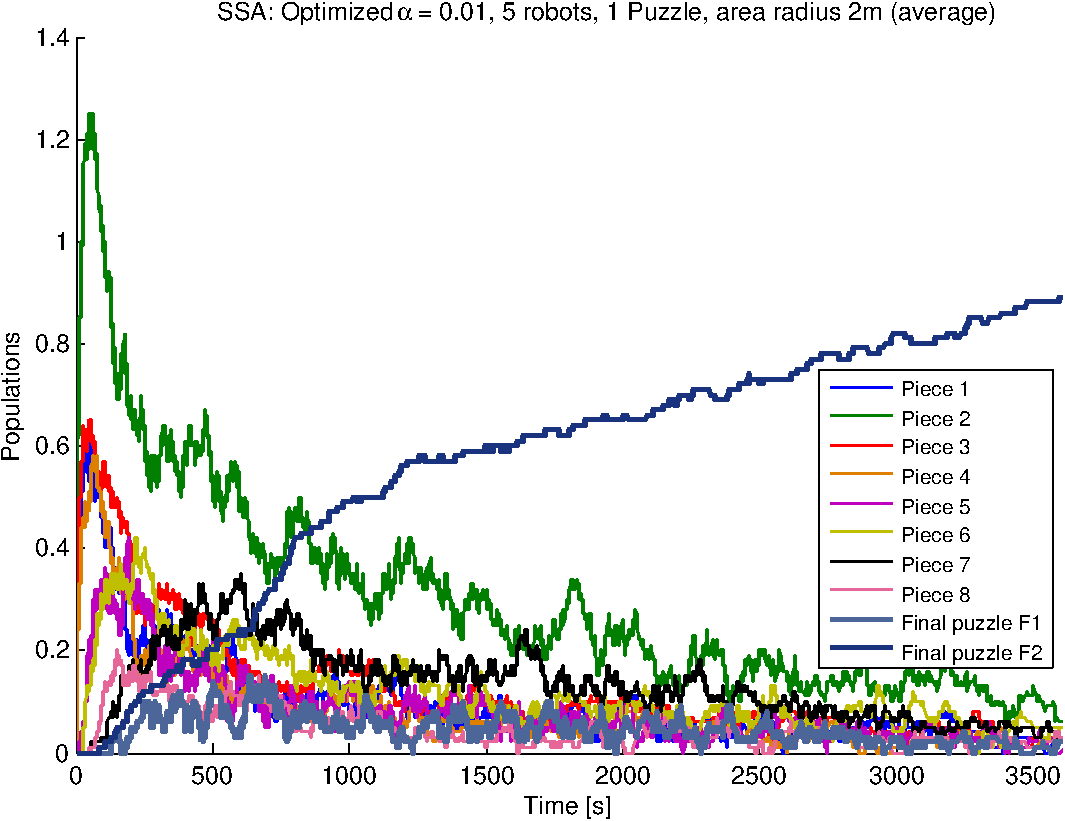
\includegraphics[width=7.2cm]{img/augm_stoch1puzzle_5robots_alpha001.pdf}
					\label{fig:stoch_augm_1puzzle:alpha001}
			 	}
		%		\: % espacement entre figures. \quad \;
				\subfigure[$\alpha = 0.5$] 
				{
					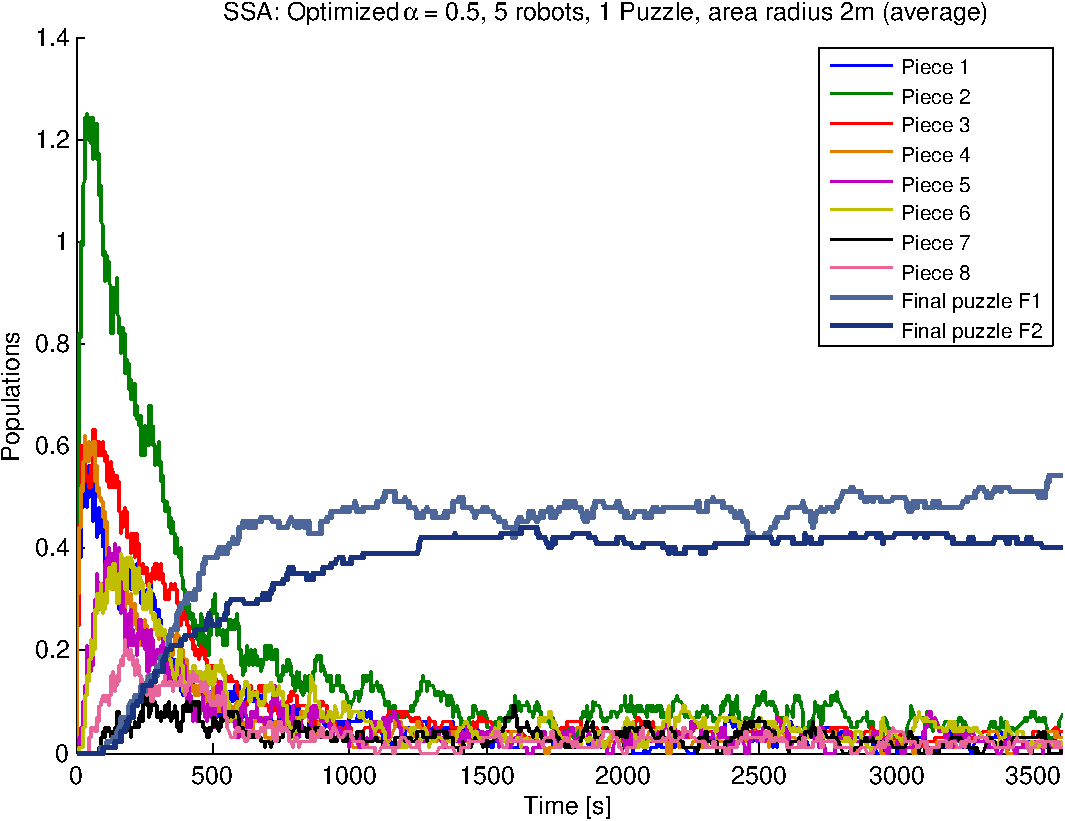
\includegraphics[width=7.2cm]{img/augm_stoch1puzzle_5robots_alpha05.pdf}
					\label{fig:stoch_augm_1puzzle:alpha05}
			 	}
		%		\: % espacement entre figures. \quad \;
				\begin{center}
					\subfigure[$\alpha = 0.99$] 
					{
						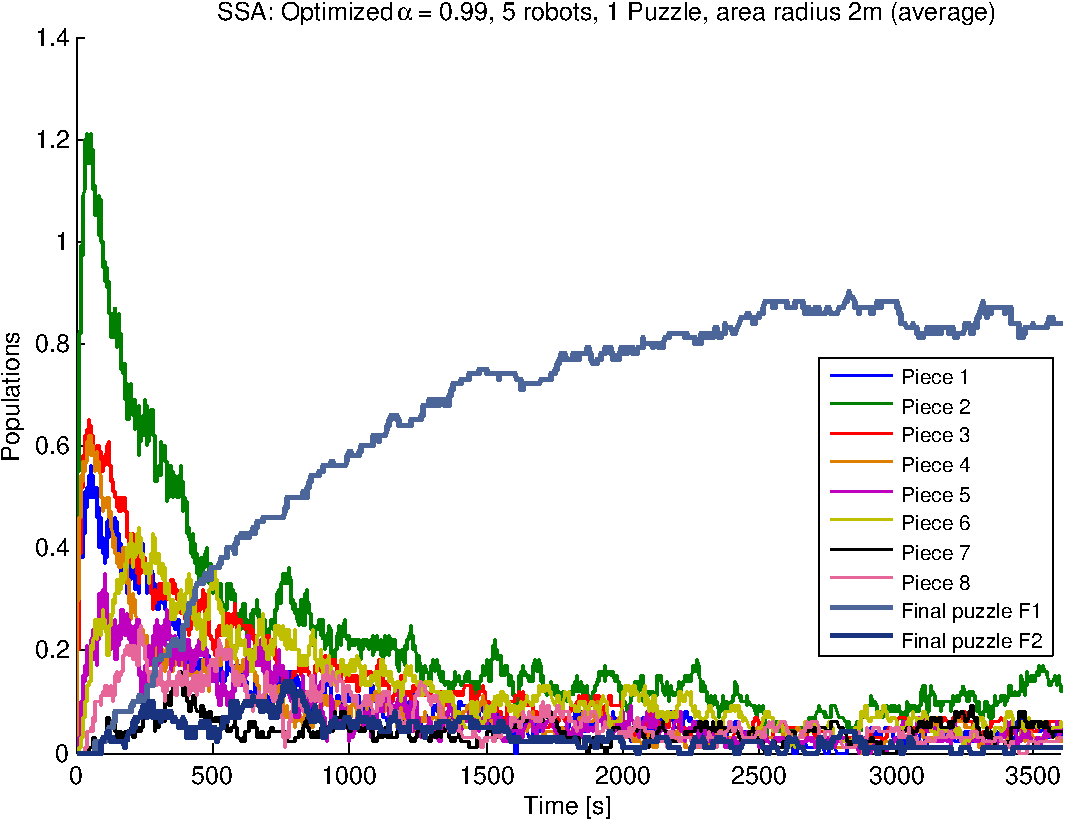
\includegraphics[width=7.2cm]{img/augm_stoch1puzzle_5robots_alpha099.pdf}
						\label{fig:stoch_augm_1puzzle:alpha099}
				 	}
					
				\end{center}
				\caption{Stochastic simulation of the Augmented system, for 1 puzzle and 5 robots.}
			\label{fig:stoch_augm_1puzzle} %Caption general
			\end{figure}
		
		According to these simulations, the optimized rates for the simplified system \eqref{eq:modified_system:reactions} translates into the same global optimized behavior when used on the complete system with robots and free pieces. It manages to create the target ratio $\alpha$ quite successfully. This is a good thing, as it shows that we have a full loop between the physical system and the optimization of the model. We see that, because of the low number of pieces available, there are still quite a lot of non final puzzles in the system. 
	% subsection stochastic_model (end)
	
	\subsection{Physical simulation} % (fold)
	\label{sub:physical_simulation}
		
		As explained earlier, we augmented the system by adding the capacity to break assemblies and grab mid-assemblies lying on the floor. We then use the optimized probabilities of Table~\ref{tab:optimized_probabilities_augmented} before running our simulations.
		
		\subsubsection{The carried pieces discrepancy} % (fold)
		\label{ssub:the_carried_pieces_discrepancy}
		
		Our first result is an experiment with $\alpha=0.01$, using 5 robots and 5 pieces. We run 100 experiments, using the same methodology as explained in Section~\ref{ssub:experiment_3_5_pieces_and_5_robots_final_puzzles_f1_and_f2}, for a maximum of 10 minutes. The results are shown in Figure~\ref{fig:img_augm_res1puzzle_5robots}.
		
		\begin{figure}[h]
			\centering
				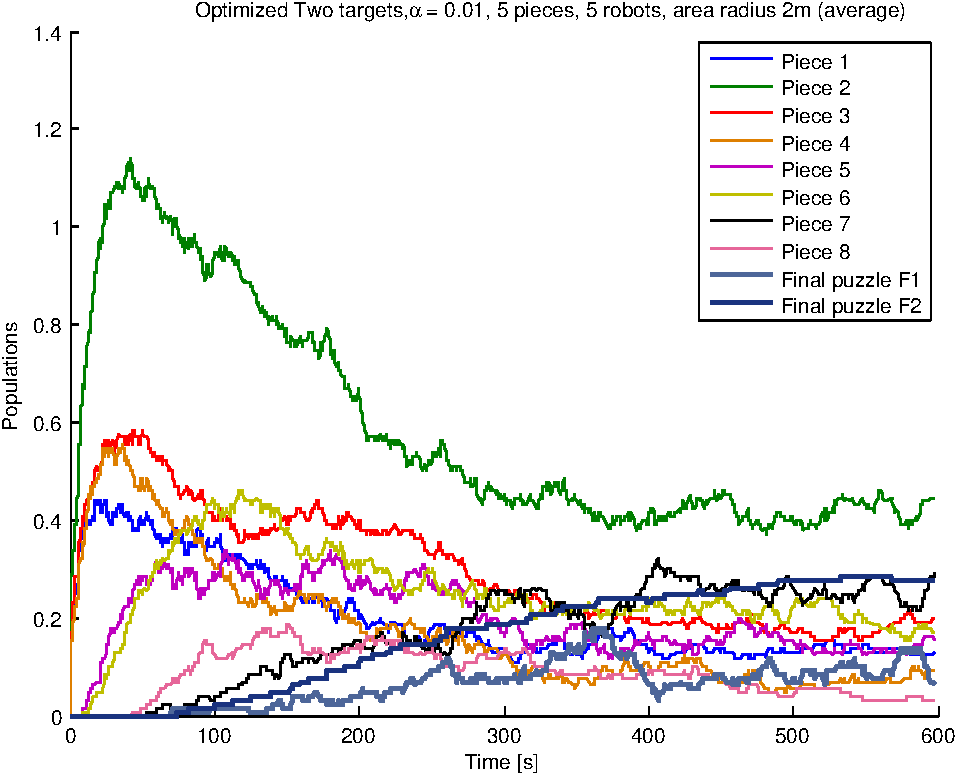
\includegraphics[width=8cm]{img/augm_res1puzzle_5robots_alpha001.pdf}
			\caption{Results of the augmented system with optimized rates for $\alpha=0.01$. Problem of carrying of pieces.}
			\label{fig:img_augm_res1puzzle_5robots}
		\end{figure}
		
		This is quite disappointing, as it does not converge to our desired values, even if we do not run the system for a long time. The biggest problem is the amount of free piece 2: they are more abundant than final assemblies.
		
		Studying visually the behavior in simulation, we discovered that this problem is due to the re-carrying of pieces dropped during a disassembly. When few robots are available, the time till a piece is carried again can be in the same order of magnitude than the time between two assemblies. Yet when constructing our model for the optimization, we assumed that the pieces would be carried very quickly (Section~\ref{sub:changes_on_our_models}). This hypothesis is thus pretty important as its effect shows it here.
		
		In order to correct that, we add 3 robots to the arena, which ensure that the time to re-carrying of pieces is small.
		We then compare the results of this new physical simulation to the stochastic simulation of the same experiment in Figure~\ref{fig:img_augm_stochphys_alpha001}. Again we do 100 experiments, of 10 minutes each for a target value $\alpha=0.01$.

		\begin{figure}[h]
			\centering
				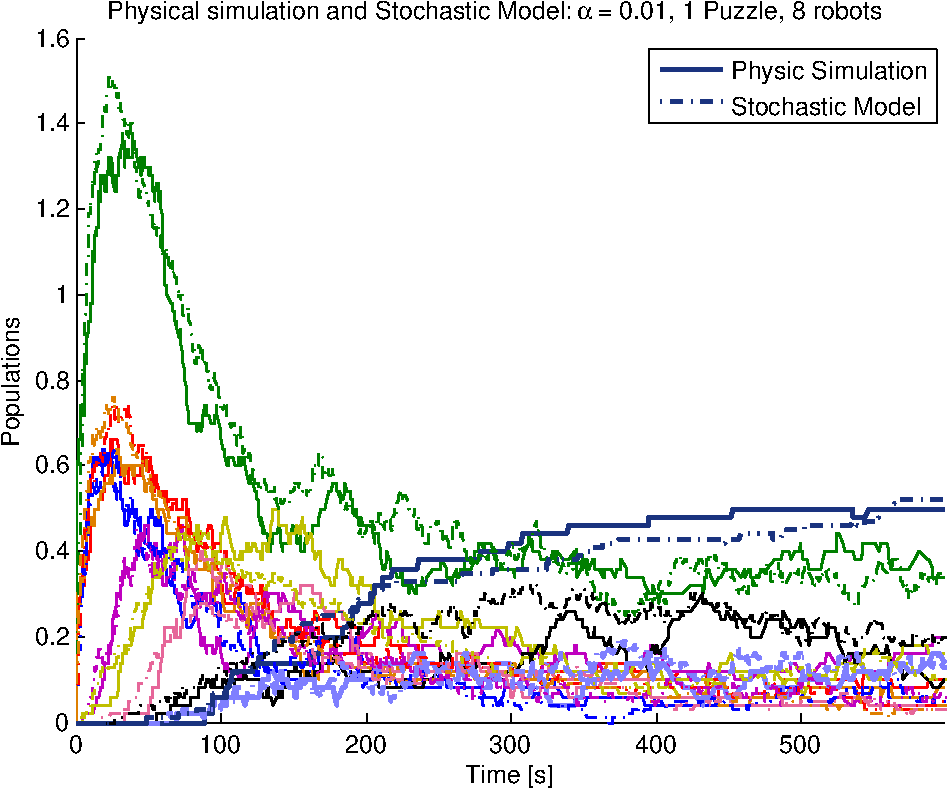
\includegraphics[width=10cm]{img/augm_stochphys_alpha001.pdf}
			\caption{Comparison between physical augmented system and stochastic model for $\alpha = 0.01$.}
			\label{fig:img_augm_stochphys_alpha001}
		\end{figure}
		
		The results between the physical and the stochastic simulations are comparable but differ slightly:
		
		\begin{my_itemize}
			\item The rates of convergence up to 9 minutes are of the same order. The stochastic model fits correctly the physical simulation.
			\item After 9 minutes, the stochastic model continues to converge towards its equilibrium, as expected from Figure~\ref{fig:stoch_augm_1puzzle:alpha001}, but the physical simulation saturates to a sub-optimal value. The amount of free pieces 2 is kept pretty high, without assembling to create the desired final puzzle F2. 
		\end{my_itemize}
		
		When observing visually the behavior of the system, it appears that two scenarios are occurring:
		\begin{my_enumerate}
			\item The system builds a final puzzle F2. As the backward rate from this puzzle is very slow, it is kept complete till the end of the simulation.
			\item The system builds a final puzzle F1. According to our rates, it should disassemble back till a convergence to F2. Unfortunately this disassembly does not work that well. Several problem arise:
				\begin{my_itemize}
					\item When F1 disassemble, it is very likely that the lying free piece 2 is taken and assembled back into a new F1. The problem comes from spatial constraints: the piece is dropped near the current robot.
					\item If F1 disassembles, we end up with an assembly 7 and an initial piece 2. The backward rate to disassemble 7 is low, which posses a problem in our case. We think that because 7 stays alive for some time, it has more chances to assemble back with the piece 2 than disassemble further, because of the spatial problem we presented.
				\end{my_itemize}
		\end{my_enumerate}
		
		There seems to be an even distribution between the two scenarios, the second of them impeding the capacity of the system to converge to the target ratio. We would need to do an iterative process to bring back this difference to the model level, in order to get optimized rates taking it into account.
		% subsubsection the_carried_pieces_discrepancy (end)
		
		\subsubsection{Other target ratios $\alpha$} % (fold)
		\label{ssub:other_target_ratios_alpha_}

			
			See Figure~\ref{fig:img_augm_stochphys_otheralpha} for the two other target ratio and their comparison with the stochastic model. The methodology is again the same, we perform 100 experiments of 20 minutes.
			
			We see that we closely fit the predicted data, but that the physical simulations converge to sub-optimal values in both cases. Again the ``mobility'' between assemblies in the real system is much smaller than in the model. This prevents a good convergence to theoretical values over time.
			
			
				\begin{figure}[h!]
					\centering
					\subfigure[$\alpha = 0.5$] 
					{
						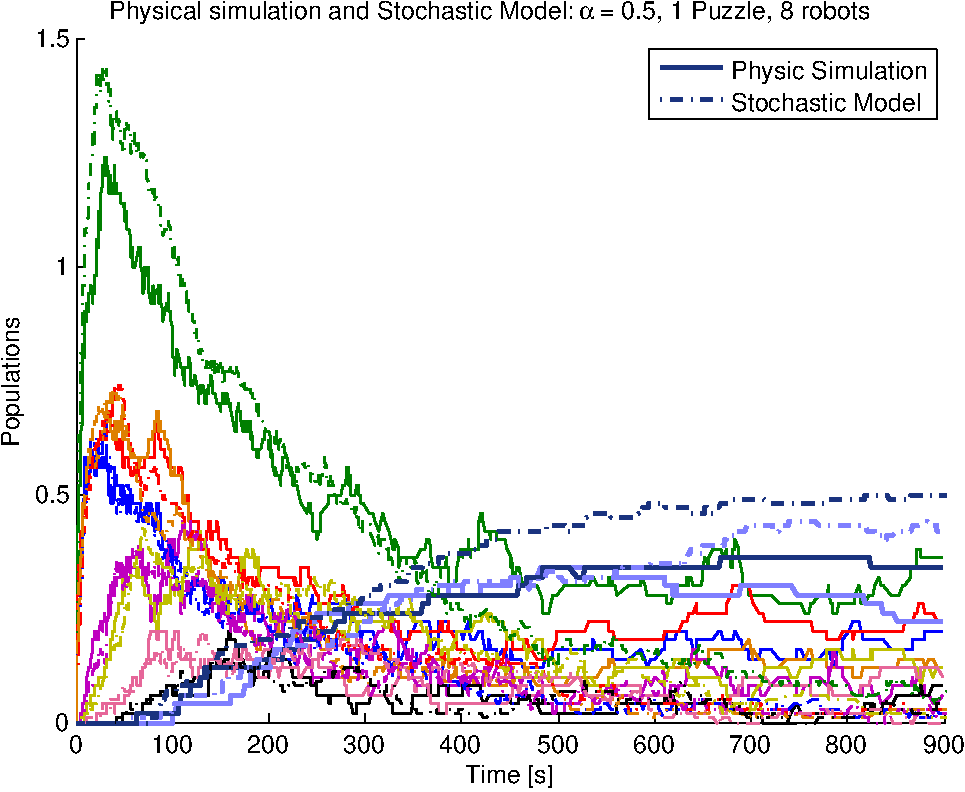
\includegraphics[width=10cm]{img/augm_stochphys_alpha05.pdf}
						\label{fig:img_augm_stochphys_otheralpha:alpha05}
				 	}
			%		\: % espacement entre figures. \quad \;
					\subfigure[$\alpha = 0.99$] 
					{
						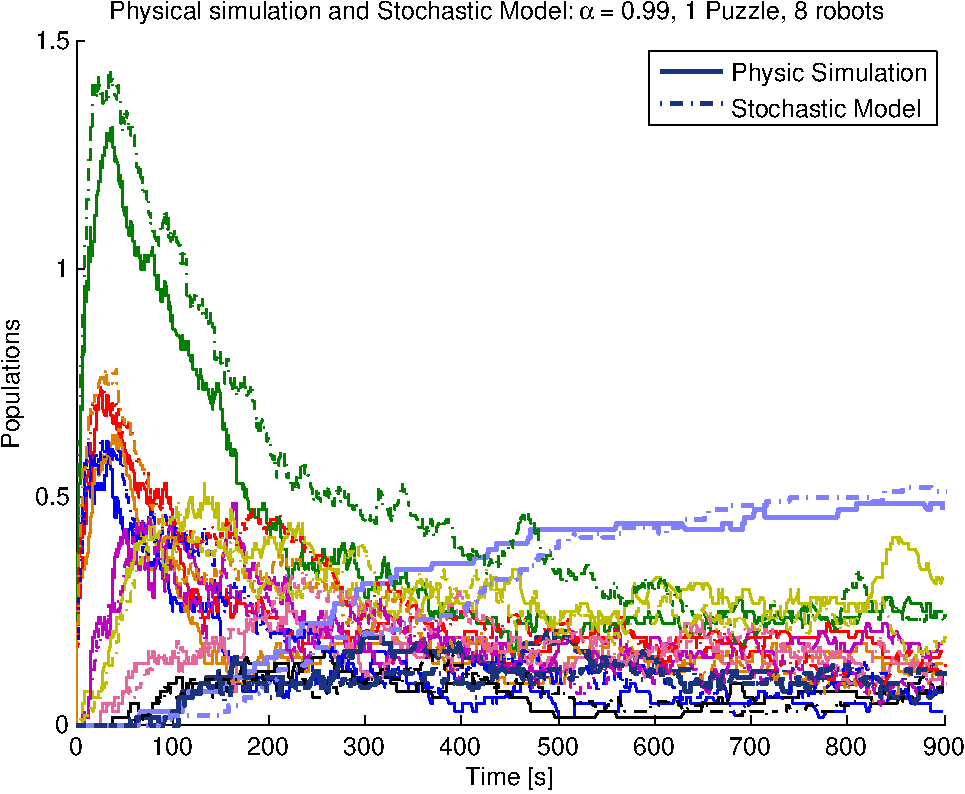
\includegraphics[width=10cm]{img/augm_stochphys_alpha099.pdf}
						\label{fig:img_augm_stochphys_otheralpha:alpha099}
				 	}
			%		\: % espacement entre figures. \quad \;
					\caption{Augmented system results for $\alpha=0.5$ and $\alpha=0.99$. Comparison with the stochastic model.}
				\label{fig:img_augm_stochphys_otheralpha} %Caption general
				\end{figure}
				
			Even though the yield is bad, it has to be remarked that the ratios $\alpha$ are successfully enforced by the optimized rates. This might point out that the problem does not come from the dynamics directly but from the small amount of pieces available. Further tests with bigger amount of pieces would be needed, but we are limited by simulation constraints for the time being.
			
		% subsubsection other_target_ratios_alpha_ (end)
	% subsection physical_simulation (end)
	
	\subsection{Implications} % (fold)
	\label{sub:implications}
		We saw that it was possible to use the rates we optimized in a simplified mathematical model to map onto the physical system. It successfully created the desired ratios of final puzzles, even though the dynamics of interactions between robots is quite complex and random. The Top-down approach of our framework is thus valid and promising even at this early stage.
		
		However, some differences can have big impacts. Small copy numbers can disturb the convergence, and the non-spatiality assumption can have bad effects when our physical system does not manage to satisfy it. We think that our approach is still worthy of interest and leads to insightful results, especially theoretically. It would need some tuning in order to map correctly the theoretical optimized probabilities onto the physical system. Unfortunately, this would have to be done in a further work.
	% subsection implications (end)
% section augmentation_results_and_implications (end)